\documentclass[a4paper,titlepage]{article}
\usepackage[utf8]{inputenc}
\usepackage[T1]{fontenc}
\usepackage[portuges]{babel}
% setspace - \doublespace \onehalfspace
% fullpage - ??
\usepackage{verbatim,url}
\usepackage[dvips]{graphicx}
\usepackage[bf]{subfigure}
\usepackage[bf]{caption}
\usepackage{amsmath, amssymb, algorithm, algorithmic,fullpage,setspace}
\usepackage{mathtools,empheq}
\usepackage[pagebackref=true,breaklinks=true,letterpaper=true,colorlinks,bookmarks=false]{hyperref}
\usepackage{multirow}
\usepackage{xspace}
\usepackage{array}

\newtheorem{definition}{Defini��o}
\newtheorem{theorem}{Teorema}
\newtheorem{notation}{Nota��o}
\floatname{algorithm}{Algoritmo}

\newenvironment{changemargin}[2]{\begin{list}{}{
   \setlength{\topsep}{0pt}\setlength{\leftmargin}{0pt}
   \setlength{\rightmargin}{0pt}
   \setlength{\listparindent}{\parindent}
   \setlength{\itemindent}{\parindent} \setlength{\parsep}{0pt plus 1pt}
   \addtolength{\leftmargin}{#1}\addtolength{\rightmargin}{#2}
}\item }{\end{list}}

%%%%%%%%%%%%%%%%%%%%%%%%%%%%%%%%%%%%%%%%
% You have many versions of the macro \draftnote{My note}. 
% The first version puts notes (My note in the example)
% into the margin. The others insert within the document. 
% Toggle the empty definitions to hide all draft notes.

\newcommand{\draftnote}[1]{\marginpar{\tiny\raggedright\textsf{\hspace{0pt}#1}}}
%\newcommand{\draftnote}[1]{}
%
% This one is just for the comments for in-line text.
\newcommand{\indraftnote}[1]{\textcolor{blue}{\texttt{\footnotesize [#1]}}}
%\newcommand{\indraftnote}[1]{}

\newcommand{\todo}[1]{\indraftnote{todo: #1}}
%\newcommand{\todo}[1]{}
\usepackage{listings} % better verbatim env for sketching outlines/lists
\lstset{
basicstyle=\small,
columns=flexible,
breaklines=true
}

% Uncomment to eliminate draft text
\lstnewenvironment{draft}{ } { }
%\newenvironment{draft} {\expandafter\comment} {\expandafter\endcomment}   % Empty 

\newcommand{\scilab}{\textsc{Scilab}}
\newcommand{\matlab}{\textsc{Matlab}}
\newcommand{\sip}{SIP}
\newcommand{\animal}{AnImaL}
\newcommand{\eg}{{p.\ ex.}}
\newcommand{\etc}{{\it etc}}
\newcommand{\ie}{{\it i.e.}}
\newcommand{\etal}{{\it et al.}}
\newcommand{\id}{\text{\emph{Id}}}
\newcommand{\dof}{\textsc{dof}}
\newcommand{\ransac}{\textsc{ransac}}
\newcommand{\sift}{\textsc{sift}}
\newcommand{\svd}{\textsc{svd}}
\newcommand{\sfm}{\textsc{sfm}}

\newcommand{\Gama}{\boldsymbol{\Gamma}}
\newcommand{\gama}{\boldsymbol{\gamma}}
\newcommand{\bsigma}{\boldsymbol{\sigma}}
%\newcommand{\Gama}{\Gamma}
%\newcommand{\gama}{\gamma}
\newcommand{\T}{\boldsymbol{T}}
\newcommand{\N}{\mathbf{N}}
\newcommand{\NSurface}{\mathbf{N}}
\newcommand{\Nlocal}{\overline{\N}} % normal in local coordinates
\newcommand{\balpha}{\boldsymbol{\alpha}}
\newcommand{\tDt}{t+\Delta t}
\newcommand{\bpsi}{\boldsymbol{\boldsymbol{\psi}}}
\newcommand{\bp}{\mathbf p}
\newcommand{\deldt}[1]{\frac{\partial#1}{\partial t}}
\newcommand{\ddt}[1]{\frac{d #1}{dt}}
\newcommand{\delds}[1]{\frac{\partial#1}{\partial s}}
\newcommand{\mybar}[1]{\overline{#1}}
\newcommand{\norm}[1]{\|#1\|}
\newcommand{\I}{\mathbf{I}}
\newcommand{\brho}{\boldsymbol{\rho}}
\newcommand{\lightrgb}{\boldsymbol{l}}
\newcommand{\B}{\boldsymbol{B}}
\renewcommand{\t}{\boldsymbol{t}}
\newcommand{\n}{\boldsymbol{n}}
\renewcommand{\b}{\boldsymbol{b}}
\newcommand{\e}{\boldsymbol{e}}
\newcommand{\f}{\boldsymbol{e}_3}
\newcommand{\ff}{\mathbf{f}}
\newcommand{\hf}{\boldsymbol{\hat{f}}}
\newcommand{\g}{\boldsymbol{g}}
\newcommand{\G}{\boldsymbol{G}}
\newcommand{\bc}{\boldsymbol{c}}
\newcommand{\Curve}{\Gamma}
%\newcommand{\X}{\boldsymbol{X}}
%\newcommand{\x}{\boldsymbol{x}}
\newcommand{\X}{\mathbf{X}}
\newcommand{\x}{\mathbf{x}}
\newcommand{\tilx}{\tilde x}
\newcommand{\tily}{\tilde y}
\newcommand{\tilgama}{\tilde \gama}
\newcommand{\ugama}{\hat{\gama}} %unit gama
\newcommand{\br}{\bar r}
\newcommand{\Kc}{\mathbf K_c}
\newcommand{\Kim} {\mathcal K_{im}}
\newcommand{\lepi}{\mathbf r}
\newcommand{\itan}{\tan^{-1}}
\newcommand{\uu}{\xi}
\newcommand{\buu}{\bar \uu}
\newcommand{\bvv}{\bar \vv}
\newcommand{\vv}{\eta}
\newcommand{\VV}{\mathbf{V}} % translational velocity
\newcommand{\VVspeed}{V} % translational velocity
\newcommand{\field}{\boldsymbol\chi}
\newcommand{\ufield}{\hat{\boldsymbol{\chi}}}
\newcommand{\fieldc}{\chi} % field component
\newcommand{\transl}{\mathcal{T}}
\newcommand{\rot}{\mathcal{R}}
\newcommand{\albedo}{\alpha}
\newcommand{\depth}{\rho}      % depth as z
\newcommand{\udepth}{{\hat{\rho}}} % depth along ray
\newcommand{\ttransl}{\T} % translation tangent
\newcommand{\surface}{\mathcal{M}} % surface/manifold
\newcommand{\surf}{\mathcal{M}} % surface/manifold short
\newcommand{\jacm}{\mathtt{J}} % Jacobian matrix
\newcommand{\xbar}{\bar x}
\newcommand{\ybar}{\bar y}
\newcommand{\zbar}{\bar z}

\newcommand{\bdelta}{\boldsymbol \delta}
%\newcommand{\X}{\boldsymbol{X}}
%\newcommand{\x}{\boldsymbol{x}}
%\newcommand{\X}{\mathbf{X}}
%\newcommand{\x}{\mathbf{x}}
\newcommand{\boldu}{\mathbf{u}}
\newcommand{\boldv}{\mathbf{v}}
\newcommand{\boldw}{\mathbf{w}}
\newcommand{\tgtveloc}{\tilde\alpha} % real tangential velocity
\newcommand{\mccn}{\textsc{mccn}\xspace}

\newcommand{\argmin}{\operatornamewithlimits{argmin}}
\newcommand{\argmax}{\operatornamewithlimits{argmax}}
\newcommand{\avg}{\operatornamewithlimits{avg}}

\begin{document}

\begin{titlepage}
\begin{changemargin}{-0.5cm}{-1cm}
\renewcommand{\title}{%
  {\LARGE Assinaturas de Sinais Geométricos}\\[4pt]
  {\LARGE para Reconstrução 3D Multiperspectiva de Curvas e Superfícies}
}
\renewcommand{\author}{Clêuber Eduardo do Nascimento Silva}
%\renewcommand{\date}{\today}
\newcommand{\info}{%
  \raisebox{4pt}[-4pt]{%
  
\includegraphics[height=1.3cm]{figs/logo-iprj2.eps} 
  \hspace{0.1in}
  }

  Laboratório de Visualização\\
  Laboratório de Tecnologia da Informação\\
  Instituto Politécnico -- IPRJ\\
  Universidade do Estado do Rio de Janeiro\\[1.5cm]

  Nova Friburgo, 15 de Novembro de 2020\\[1.5cm]

  \textbf{Projetos Relacionados}\\[4pt]
   FAPERJ Jovem Cientista do Nosso Estado E25/2014 204167\\
   FAPERJ APQ1 01/09335-8\\
   FAPERJ E28/2014/204747\\
   UERJ Prociência 2014--2017
}

%% Abstand zwischen oberem Blattrand und Titel.
\newlength{\topToTitle} 
\setlength{\topToTitle}{30pt}

%% Abstand zwischen linkem Blattrand und Titel.
\newlength{\leftToTitle} 
\setlength{\leftToTitle}{-50pt}

%% Abstand zwischen Titel und Info-Feld.
\newlength{\titleToInfo} 
\setlength{\titleToInfo}{7cm}

%% \myTextWidth erhoehen, um Info-Feld weiter nach Rechts zu schieben.
\newlength{\myTextWidth}
\setlength{\myTextWidth}{\textwidth}
\advance\myTextWidth by 1.5cm


\thispagestyle{empty}
\vspace*{\topToTitle}
\begin{minipage}{\myTextWidth}
  \sffamily
  \hspace*{\leftToTitle}\begin{minipage}{60cm}
    \Large\textbf{Plano de Trabalho de Doutorado}\\[1.5cm]
    \title\\[1.5cm]
    \author
  \end{minipage}\\

  %% \enlargethispage{} um ggfs. Titel und Info-Feld weiter
  %% auseinanderziehen zu koennen.
  \vspace*{\titleToInfo}

  \begin{minipage}{\textwidth}
    \flushright
    \info
  \end{minipage}
\end{minipage}%
\end{changemargin}
\end{titlepage}


%\tableofcontents
%\contentsline {section}{Refer\^{e}ncias}{16}
%\newpage
%\doublespacing
%\onehalfspacing
%

%%%%%%%%%%%%%%%%%%%%%%%%%%%%%%%%%%%%%%%%%%%%%%%%%%%
% TODO  TODO TODO 
%  - italico em spots e sub-arrays
%  - XXX
%  - @@@
%%%%%%%%%%%%%%%%%%%%%%%%%%%%%%%%%%%%%%%%%%%%%%%%%%% 

\section{Contextualização}

O presente plano de pesquisa se refere a atividades propostas para o aluno
Cleuber Silva, a serem realizadas a nível de doutorado no Instituto
Politécnico -- IPRJ/UERJ, Departamento de Modelagem Computacional.
Pretende-se trabalhar em conjunto com dois orientadores, os quais seriam prof.\
Ricardo Fabbri, do laboratório de visualização, e o prof.\ Francisco Duarte
Moura Neto, do laboratório de tecnologia da informação (LTI), juntando-se os
aspectos ativos recentemente das pesquisas de ambos. Pretende-se trabalhar em
conjunto com outros grupos de pesquisa além desses dois laboratórios dentro do
IPRJ, bem como outros pesquisadores no IMPA e em outras instituições em
colaboração internacional na realização de projetos e publicação de artigos.
Dentre as instituições internacionais envolvidas, tem-se: University of
Minneapolis (com Peter Olver), Brown University (com Benjamin Kimia) e
University of Liverpool (com Peter Giblin).

\section{Introdução}


Na presente década está se presenciando um nível de investimentos sem
precedentes em ecosistemas de tecnologia para modelagem 3D de fenômenos
usando-se múltiplas imagens adquiridas por uma câmera em diferentes posições,
múltiplas câmeras, ou vídeo~\cite{AppleKeynote:2018}. % A Expand here on explicit applications and citations
% - mention concrete appso ok
% - mention hot techs that have been developed, then link to next sentence
Esse impacto cada vez maior da visão computacional 3D se deve em grande parte a
tecnologias de \emph{structre from motion} (SfM) desenvolvidas na década
passada, a qual possibilitou novas ferramentas para resolver problemas chave de
forma robusta e automática. No entanto, o vasto potencial das tecnologias 3D
permanece ainda inexplorado, em parte devido à rentabilidade de aplicações mais
simples e imediatas, e em parte devido a limitações da tecnologia evidentes
na medida em que aplicativos práticos são desenvolvidos, como realidade
aumentada~\cite{AppleKeynote:2018}. Pode-se afirmar que tais limitações se devem
a três problemas centrais: o uso de geometria projetiva clássica de pontos, sem 
a geometria diferencial necessária para modelar estruturas mais gerais; o uso
sub-ótimo de múltiplas imagens; e a necessidade de modelos 3D mais
estruturados.

O grupo de pesquisa do prof.\ Ricardo Fabbri tem tradição em um novo paradigma
fotogramétrico para a reconstrução 3D de objetos rígidos e não-rígidos a partir
de múltiplas imagens e
vídeo~\cite{Fabbri:Kimia:IJCV2016,Fabbri:PhD:2010,Fabbri:Giblin:Kimia:ECCV12,Fabbri:Kimia:EMMCVPR2005,Fabbri:Kimia:CVPR10,Usumezbas:Fabbri:Kimia:CVPR:2017,Usumezbas:Fabbri:Kimia:ECCV16}.
A pesquisa do prof.\ Fabbri tem como objetivo suplantar as limitações
supracitadas da tecnologia usual de reconstrução 3D, a qual é baseada em (e
limitada por) pontos de interesse. Uma das formas para se atingir esse objetivo
é empregando-se a informação disponível em curvas perceptuais em imagens,
através de um modelo 3D com progressivos níveis de detalhe baseado no chamado
\emph{3D curve sketch} (esboço 3D de curvas) e o \emph{3D curve drawing}
(desenho 3D de curvas). Tendo obtido um esboço inicial dos objetos 3D através do
casamento de curvas ao longo das múltiplas imagens, o modelo 3D pode ser
refinado em um grafo de curvas, similar a um desenho 3D. Superfícies podem ser
estendidas sobre esse desenho 3D para gerar uma reconstrução detalhada e
robusta a iluminação. Além da proposta do paradigma baseado em curvas, prof.\
Fabbri e colaboradores foram os primeiros a introduzir a ténica
CAD chamada \emph{Lofting} de interpolação de curvas por superfícies à visão
computacional em uma versão automática.

Este projeto é um segundo projeto de doutorado que objetiva unir a pesquisa em
aprendizagem de máquina baseada em difusão em grafos -- proveniente da
colaboração entre os orientadores prof.\ Ricardo Fabbri e prof.\ Francisco
Duarte Moura neto --  com a pesquisa específica em reconstrução 3D do prof.\
Fabbri. O primeiro projeto nesta linha foi da aluna de doutorado Juliana
Ventura, em andamento, o qual visa melhores algoritmos para inicializar modelos
de câmera e de objetos curvilíneos com pouca textura; ou seja, visa os estágios
iniciais dos sistemas de reconstrução 3D. O presente projeto, em
contraste, visa os estágios finais de reconstrução 3D que tratam da reconstrução
3D de superfícies usando-se curvas, mais especificamente a reconstrução de
superfícies de oclusão usando-se contornos aparentes (\emph{apparent contours}).

A Figura~\ref{fig:multiview:stereo} mostra um exemplo de técnica já bem
estabelecida de reconstrução 3D de superfícies a partir de contornos de oclusão.
Estas técnicas, porém, exigem aquisição controlada (condições de estúdio).
O objetivo da pesquisa do prof.\ Fabbri é trabalhar com aquisição não-controlada.
\begin{figure}
\begin{center}
  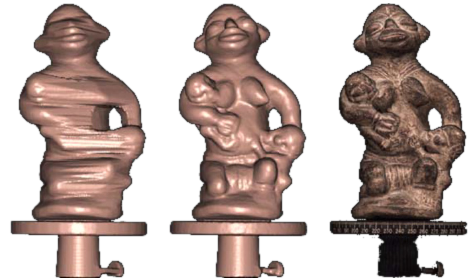
\includegraphics[width=0.5\linewidth]{figs/multiview-stereo-white.png}
\end{center}
   \caption{
A reconstrução 3D clássica a partir de perfis de superfícies~\cite{Hernandez:Schmitt:CVIU04}
fornece modelos detalhados (direita), porém exigem condições altamente
controladas de aquisição. Elas são inicializadas pelo fecho convexo visual do
objeto (esquerda), matematicamente o envelope de uma família de superfícies retroprojetadas a
partir de uma família de curvas 2D (obtidas filmando-se o contorno do objeto a
partir de múltiplas perspectivas).
}
\label{fig:multiview:stereo}
\end{figure}


% XXX fig dos tipos de curvas

A ideia principal é capitalizar nos avanços recentes e de alto impacto
realizados pelo prof.\ Fabbri durante sua estadia no ICERM / Brown University,
ao final de 2018 e no início de 2019 como organizador do Research Cluster em
``Visão Algébrica'', onde reuniu e liderou os melhores professores visitantes e seus alunos
de doutorado para investigar os problemas desta pesquisa. No início de 2019, o
grupo organizado pelo prof.\ Fabbri conseguiu levar consigo o ex-aluno de
mestrado do IPRJ David da Costa de Pinho aos Estados Unidos, e sua tese de mestrado desenvolvida no
IPRJ teve grandes desdobramentos. Durante a estadia do prof. Fabbri no ICERM,
um dos professores que estavam participando do programa \emph{Nonlinear
Algebra} ao final de 2018 foi o pesquisador Peter Olver, um matemático dentre os
mais produtivos do mundo, que trabalha também em visão computacional e é
considerado um dos expoentes dos invariantes diferenciais e grupos de Lie em
EDPs. Peter Olver e prof.\ Fabbri iniciaram uma colaboração mais intensa em 2020, quando Olver enviou
dois preprints para o prof.\ Fabbri abordando o problema de reconstrução 3D
por técnicas de invariantes diferenciais. Em especial, os preprints de Olver
formulam o problema da reconstrução 3D de superfícies como um problema da
reconstrução 3D de sinais através de um conjunto de \emph{assinaturas} desses
sinais. Um problema específico que se iniciou junto ao aluno Clêuber é a
reconstrução 3D de superfícies através da assinatura geométrica gerada por uma
família de curvas em um vídeo. Tal problema já havia sido abordado por
Fabbri~\cite{Fabbri:Kimia:IJCV2016}, porém a sofisticação matemática de Olver
será necessária para levar essas técnicas adiante, permitindo
incorporar algumas técnicas de reconstrução 3D de superfícies em um sistema
prático de fotogrametria digital.

Com o acabouço de aprendizagem de máquina trabalhado entre os prof.\ Fabbri e
prof.\ Moura Neto nos últimos anos, que envolve difusão em grafos e Teoria de
Padrões, juntamente com as técnicas do prof.\ Peter Olver, será possível
alavancar o \emph{expertise} de equações diferenciais do prof.\ Moura Neto aos problemas de
reconstrução 3D trabalhados no grupo do prof.\ Fabbri. Em especial, a aplicação
prática de reconstrução 3D da superfície do mar a partir de múltiplas câmeras de
vídeo será visada, sendo muitos dos casos curvas de oclusão conforme descrito
nos preprints de Olver.


\section{Reconstrução do Desenho 3D a partir de múltiplas perspectivas}
Esta seção resume o trabalho anterior de Fabbri~\etal\ sobre o paradigma do
Desenho 3D para reconstrução de cenas (coleções de objetos) a partir de múltiplas imagens.
O fundamento matemático está presente em~\cite{fabbri2016multiview},
relacionando as propriedades diferenciais de uma curva 3D
$\Gamma(S)$, onde $\Gamma$ é um ponto 3D (possivelmente em uma curva) no sistema
de coordenadas de câmera, e $S$ é uma parametrização da curva 2D
correspondente, $\gama(s)$, onde $\gama$ é um ponto em uma imagem e $s$ é uma
parametrização da curva 3D. Usando-se a relação
$\Gamma(S) = \rho(s) \gama(S)$, onde $\rho$ é a profundidade do ponto
denotado por $\Gama$, a geometria diferencial da curva 3D
$\{
\boldsymbol{T},\boldsymbol{N},\boldsymbol{B}, K, \dot{K},\tau, G,G',G''\}$ é
relacionada à geometria diferencial da curva 
$\{\boldsymbol{\gamma},
\boldsymbol{t}, \boldsymbol{n}, \kappa, \dot{\kappa}, g, g', g'',\rho,
\rho',\rho'',\rho'''\}$, onde
$\{\boldsymbol{T},\boldsymbol{N},\boldsymbol{B}\}$ é o triedro de Frenet da
curva 3D, \ie, a tangente, normal e binormal unitário, 
$K$ e $\tau$ são as curvatura e torção da curva espacial, resp.,
$\kappa$ é a curvatura da curva numa imagem, e $G$ e $g$ são as velocidades de
parametrização das curvas 3D e 2D, resp., e onde
`` $'$  e  "  $"$ simbolizam a diferenciação relativa a um parâmetro
espacial arbitrário ($S$ ou $s$) ou parametrização por comprimento de arco,
resp. 



Note-se que $\dot{\kappa}$ e $\dot{K}$ compõe modelos intrínsecos de terceira
ordem das curvas, completo no mergulho no espaço Euclidiano 3D.
Foi demonstrado pela primeira vez por Fabbri~\etal~\cite{fabbri2016multiview} como
essas quantias estão relacionadas. Por exemplo, o vetor tangente à curva
espacial pode ser escrito como 
$\boldsymbol{T}=\rho'\boldsymbol{\gamma}+\rho g \boldsymbol{t}$, e a tangente à
curva projetada é $\boldsymbol{t}=\frac{\boldsymbol{T}-e^T_3\boldsymbol{T}
\boldsymbol{\gamma}}{||\boldsymbol{T}-e^T_3\boldsymbol{T}
\boldsymbol{\gamma}||}$,  onde $e_3^T=(0,0,1)$. Outro exemplo é que a razão das
velocidades de parametrização é uma quantia intrínseca
$\frac{g}{G}=\frac{||\boldsymbol{T}-e^T_3\boldsymbol{T}
\boldsymbol{\gamma}||}{e^T_3\boldsymbol{T}}$. Também foi demonstrada a
reconstrução de uma curva espacial (\ie, de torção não-nula) pela primeira vez na literatura.


Essas relações são muito importantes para se relacionar três ou mais imagens 
de multiplas vistas ou para reconstruir-se uma cena: foi mostrado como 
a geometria diferencial em duas vistas (tangente, curvatura, e
derivada da curvatura) reconstroem a geometria diferencial em 3D (tangente,
curvatura e torção em 3D), Figura~\ref{fig:WW1}.

{\em
  Neste projeto, focaremos na continuidade da pesquisa conjunta de Fabbri com
  Moura Neto e Olver iniciada em 2020 (após Fabbri ter conhecido Olver lno
  ICERM/Brown University), sendo esta última uma colaboração internacional de
  de grande peso que depende deste projeto de tese. Em especial, neste projeto focaremos nos problemas em
torno das equações diferenciais de movimento contínuo propostas por Fabbri~\cite{fabbri2016multiview},
as quais regem o movimento de uma curva de contorno de uma superfície suave vista por
um vídeo, em termos do movimento da câmera e da geometria da superfície.}

\begin{figure}[h]
    \centering
    a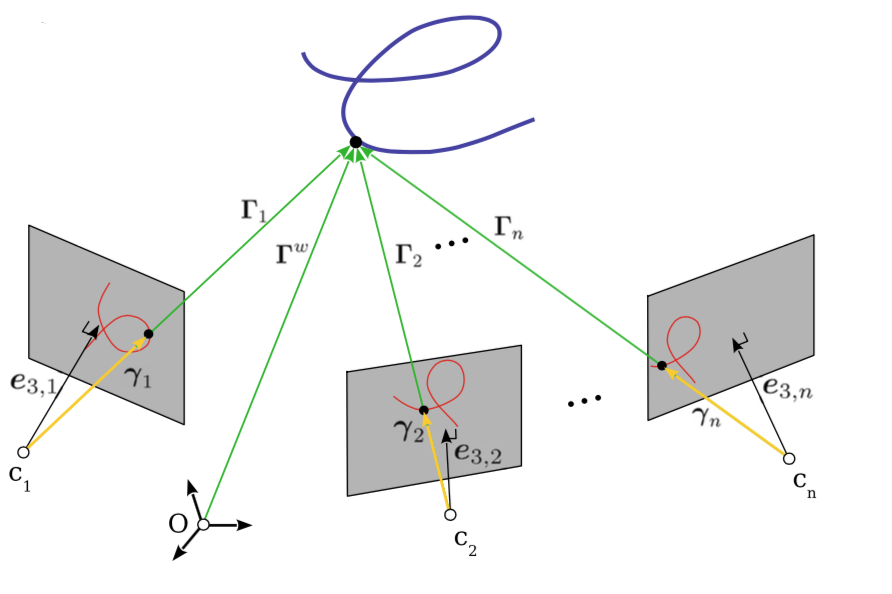
\includegraphics[width=0.45 \linewidth]{figs/FigureWW1/image51.png}\ 
    b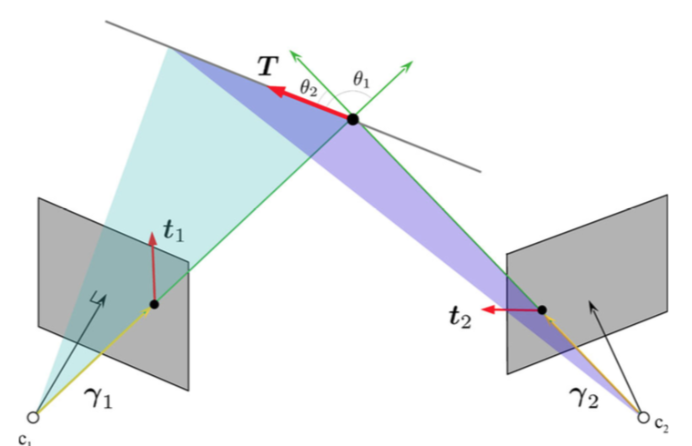
\includegraphics[width=0.45 \linewidth]{figs/FigureWW1/image211.png}
    c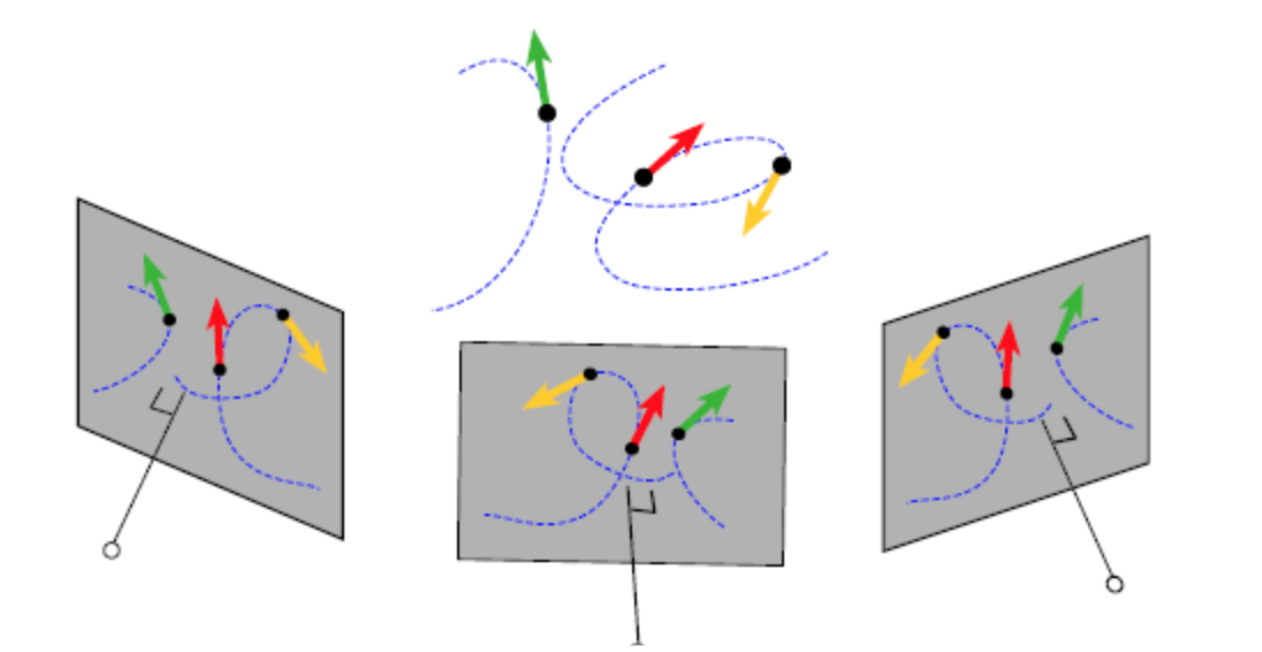
\includegraphics[width=0.45 \linewidth]{figs/FigureWW1/image18.png}
\caption{A geometria diferencial de uma curva 3D e suas projeções são
  relacionadas por equações, no caso um modelo local de primeira ordem (vetor
  tangente) em duas imagens reconstroem as tangentes no espaço tridimensional,
  e, através deste, as tangentes (modelos locais) em outras imagens.
}
    \label{fig:WW1}
    \vspace{-0.2cm}
\end{figure}
A linha de trabalhos mais práticos de Fabbri~\etal\ permite extrair um desenho
3D e superfícies acopladas, representando objetos vistos por imagens. 
As etapas desse sistema prático de reconstrução 3D são ilustradas na
figura~\ref{fig:lofting:pipeline}, sendo que nem todos os módulos ainda foram
publicados.
De maneira resumida, uma vez que as posições de câmeras tenham sido calculadas,
usando-se o trabalho desenvolvido por Fabbri junto ao ex-aluno do IPRJ David de Pinho,
e junto ao célebre matemático Peter Giblin,
cada segmento de curva em uma imagem busca porções correspondentes de curvas em
alguma outra imagem para assim hipotetizar um fragmento de curva 3D, hipótese
esta que é confirmada ou refutada reprojetando-se em outras imagens. Esse
processo resulta em um conjunto inicial desorganizado de fragmentos 3D
denominado ``esboço 3D de
curvas''~\cite{fabbri2011multiview,fabbri2016multiview},
Figure~\ref{fig:lofting:pipeline} (\emph{3D curve sketch}). Neste estágio
inicial de reconstrução, o esboço 3D de curvas sofre de erros de agrupamentos e
fragmentações, além de redundância já que a informação ainda não foi integrada
para diferentes pares de imagens, o que motivou Fabbri~\etal~\cite{usumezbas2016multiview}
a explorar a conectividade topológica  para produzir um grafo conexo de
curvas longas, denominado ``desenho 3D de curvas'', ver terceira linha na
Figura~\ref{fig:lofting:pipeline}.
\begin{figure*}
  \begin{center}
    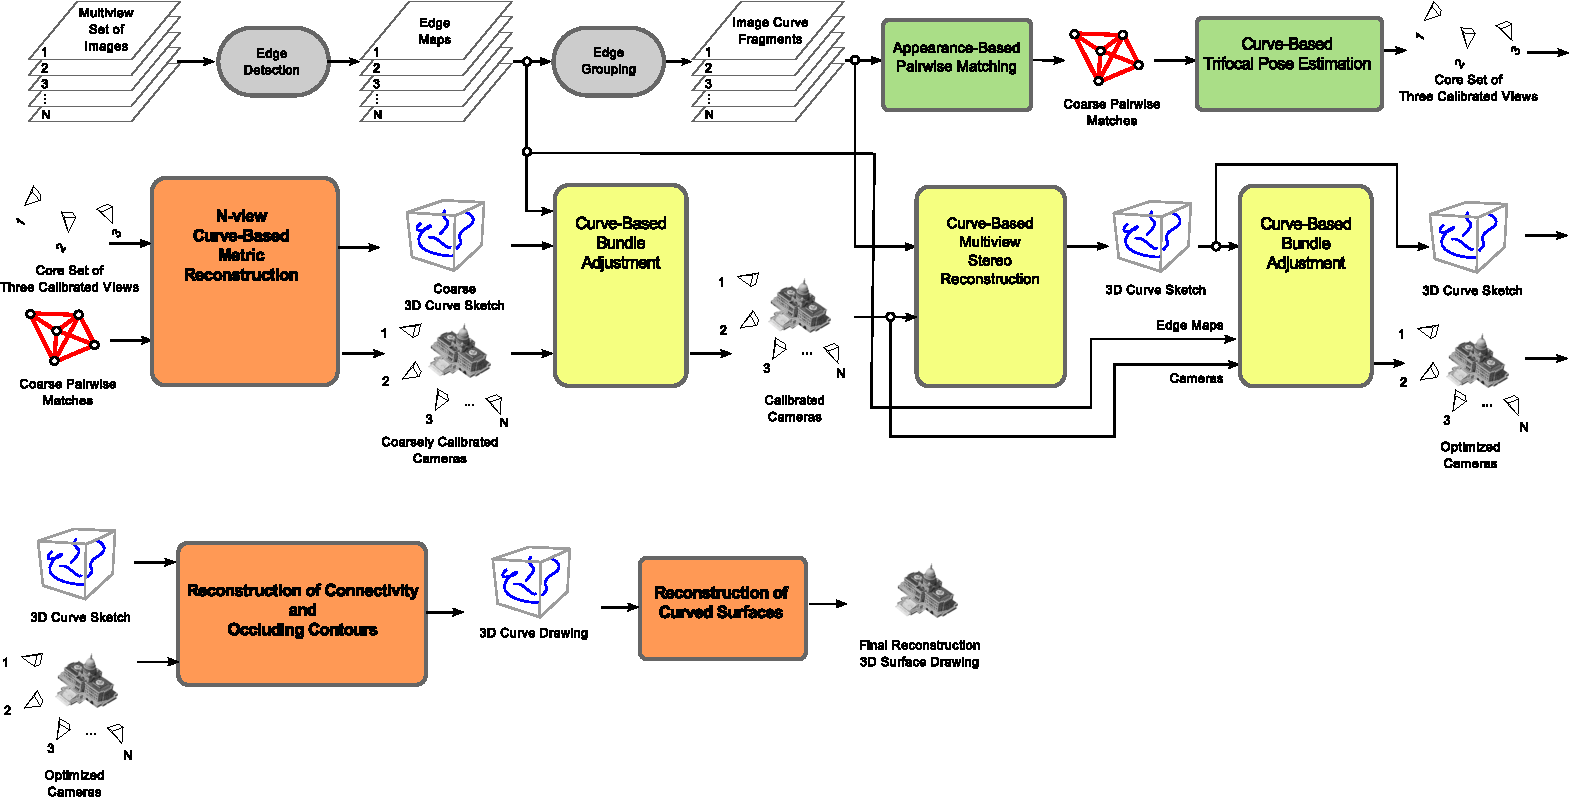
\includegraphics[width=\linewidth]{figs/mega-system-drawing-pt.pdf}
    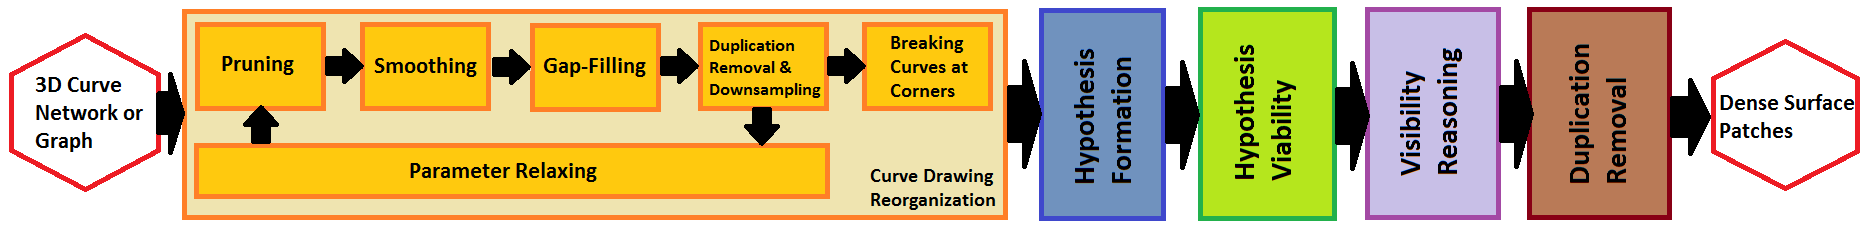
\includegraphics[width=\linewidth]{figs/lofting-pipeline.png}
  \end{center}
%  \ReduceBeforeCaptionfigspace
  \caption{Uma ilustração de um sistema completo de visão 3D baseado em curvas e
  superfícies. Muitos desses módulos ainda estão em desenvolvimento. \emph{Este
projeto se concentra nos últimos dois módulos em laranja: ``Reconstruction of
Connectivity and Occluding Contours'' e ``Reconstruction of Curved Surfaces''.}}
%  \ReduceAfterCaptionfigspace
  \label{fig:lofting:pipeline}
\end{figure*}


\section{Objetivos}

Na Figura~\ref{fig:lofting:pipeline} ilustrando os módulos do sistema de
reconstrução 3D que compõe a pesquisa do prof.\ Fabbri, \emph{pretende-se concentrar
nos últimos dois módulos em laranja: ``Reconstruction of Connectivity and
Occluding Contours'' e ``Reconstruction of Curved Surfaces''.}
usando-se ferramentas de aprendizagem de máquina baseada em
difusão em grafos e teoria de padrões, bem como invariantes diferenciais dentro
da teoria de equaçõeds diferenciais.


\subsection{Objetivo Final: Reconstrução 3D de curvas de Oclusão}

\subsubsection{Sistema prático}
Dada uma curva em uma imagem que permaneceu sem ser reconstruída após o módulo
de reconstrução 3D de curvas fixas,
as curvas que sobram podem ser perfis de surperfícies em 3D. Primeiramente, um
sistema prático poderá testar se esta curva é provieniente de uma superfície ou
não.
Testaremos primeiro essa curva como se fosse proveniente de uma superfície, e
geraremos uma reconstrução 3D de uma hipótese de superfície local. Em seguida,
testaremos essas hipóteses de que a curva é proveniente de uma superfície.
Primeiramente, essa curva em 2D precisa ser casada / rastreada ao logo de pelo
menos três imagens (por exemplo, o próximo quadro e o quadro anterior do
vídeo), Figura~\ref{fig:vj}, já que a teoria do prof.\ Fabbri prevê que três imagens são necessárias
para uma reconstrução local. Uma vez que uma hipótese de superfície em 3D
consistente com as curvas 2D é gerada, pode-se conferir se essa hipótese é
fotoconsistente com outras imagens em que esta superfície é fotografada de
maneira direta. Isso pode ser feito parametrizando-se a superfície com uma
grade, e projetando-se esta grade de pontos de forma que as múltiplas cores
interpoladas sejam minimamente consistentes ao longo de outras imagens.
Se essa hipótese de superfície local for fotoconsistente, então ela fará parte
da reconstrução 3D. A consistência global dessas hipóteses locais pode ser
inferida usando-se os modelos de aprendizagem de máquina baseados em difusão,
estudos por Moura Neto e Fabbri. 
\begin{figure}
\centering
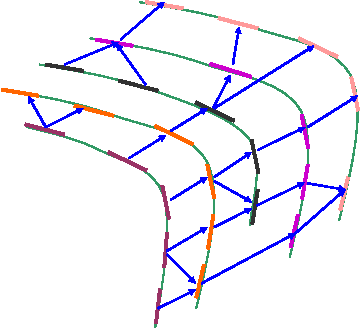
\includegraphics[scale=1]{figs/dynamic_curve_fragment-eps-converted-to.pdf}
\caption{
Hipótese local de superfície surge ligando-se uma família de curvas nas imagens.
Os segmentos de retas representam bordas de objetos nas imagens, e a família de
curvas é gerada variando-se o ponto de vista da câmera.
}
\label{fig:vj}
\end{figure}



\subsection{Objetivo Teórico: Expandir a abordagem teórica de Fabbri para outros
grupos de projeção}

A abordagem do prof.\ Fabbri para a reconstrução de curvas e superfícies permite
a reconstrução 3D tanto do objeto como da posição das
câmeras~\cite{fabbri2016multiview}. Peter Olver também publicou um
artigo recente que realiza muitas partes da mesma teoria. No entanto, apesar da
teoria de Olver ser mais geral que teoria Pesrpectiva-Euclidiana de Fabbri, os resultados
alcançados por Fabbri foram mais profundos, por exemplo sendo capaz de
determinar a reconstrução 3D da torção de curvas, bem como determinar a equação
diferenciais de curvas e contornos de oclusão. Um dos objetivos iniciais desta
pesquisa de doutorado seria procurar trazer a generalidade de Olver à
profundidade do trabalho de Fabbri.



%%%%%     \textbf{Multiview Local Consistency Network:}
%%%%%     The key idea underlying integration of reconstructions across views is the
%%%%%     detection of a common image structure supporting two reconstruction hypotheses. 
%%%%%     Two 3D local curve segments depict the same single underlying
%%%%%     3D object feature if they are supported by the same 2D image edge structures. 
%%%%%     Since the identification of common image structure can vary along the curve, it
%%%%%     must necessarily be a local process, operating at the level of a 3D local edge
%%%%%     and not a 3D curve. 
%%%%%     Two 3D edge elements (edgels) depict the same 3D structure if they 
%%%%%     receive support from the same 2D edgels in a sufficient number of views, so
%%%%%     3D-2D links between a 2D edgel to the 3D edgel it supports must be kept. Typically,
%%%%%     they share supporting image edges in many views; and the number of shared
%%%%%     supporting edgels is the measure of strength for a 3D-3D link between them.
%%%%%     
%%%%%     Formally, we define the Multiview Local
%%%%%     geometric consistency Network (MLN) as pointwise alignments $\phi_{ij}$ between 
%%%%%     two 3D curves $\Gama_i$ and $\Gama_j$: let $\Gama_i(s_i)$ and $\Gama_j(s_j)$ be
%%%%%     two points in two 3D curves, and define
%%%%%     \begin{equation}
%%%%%     S_{ij} \doteq \{v : \gama^{i,v}(s_i) \text{ and } \gama^{j,v}(s_j) \text{ share local support}\}.
%%%%%     \end{equation}
%%%%%     Then the a kernel function $\phi$ defines a consistency link between these two points,
%%%%%     weighted by the extent of multiview image support $\phi_{ij}(s_i,s_j) \doteq
%%%%%     |S_{ij}|$. When the curves are sampled, $\phi$ becomes an adjacency matrix of a
%%%%%     graph representing links between individual curve samples.
%%%%%     The implementation goes through each image edgel which votes for a 3D curve
%%%%%     point that has received support from it (see the supplementary material for
%%%%%     details).
%%%%%     
%%%%%     %\draftnote{cross check terminology w/ amir linking graphs}
%%%%%     %\draftnote{parametrized alignment to write integrals}
%%%%%     %\vspace{-0.3cm}
%%%%%     \begin{figure}
%%%%%     	%\captionsetup[subfigure]{labelformat=empty}
%%%%%     	\centering
%%%%%     	\begin{tabular}{cc}
%%%%%     %    \vspace{-0.3cm}
%%%%%     		\multirow{2}[2]{*}[20mm]{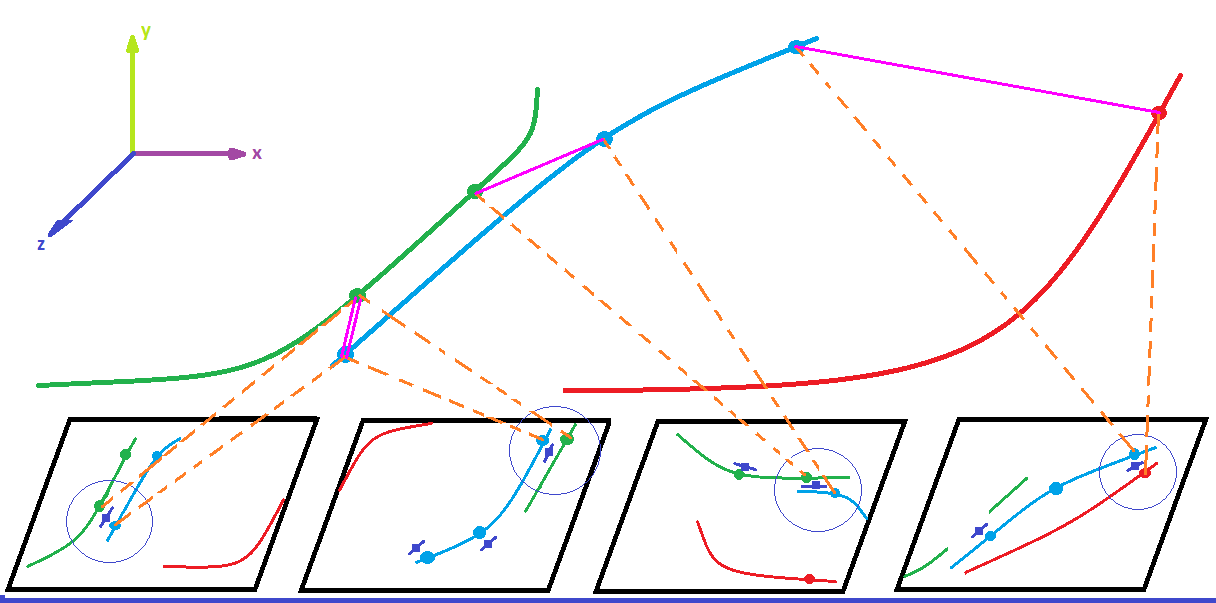
\includegraphics[width=0.75\linewidth]{figs/master-figure.png}} &
%%%%%     		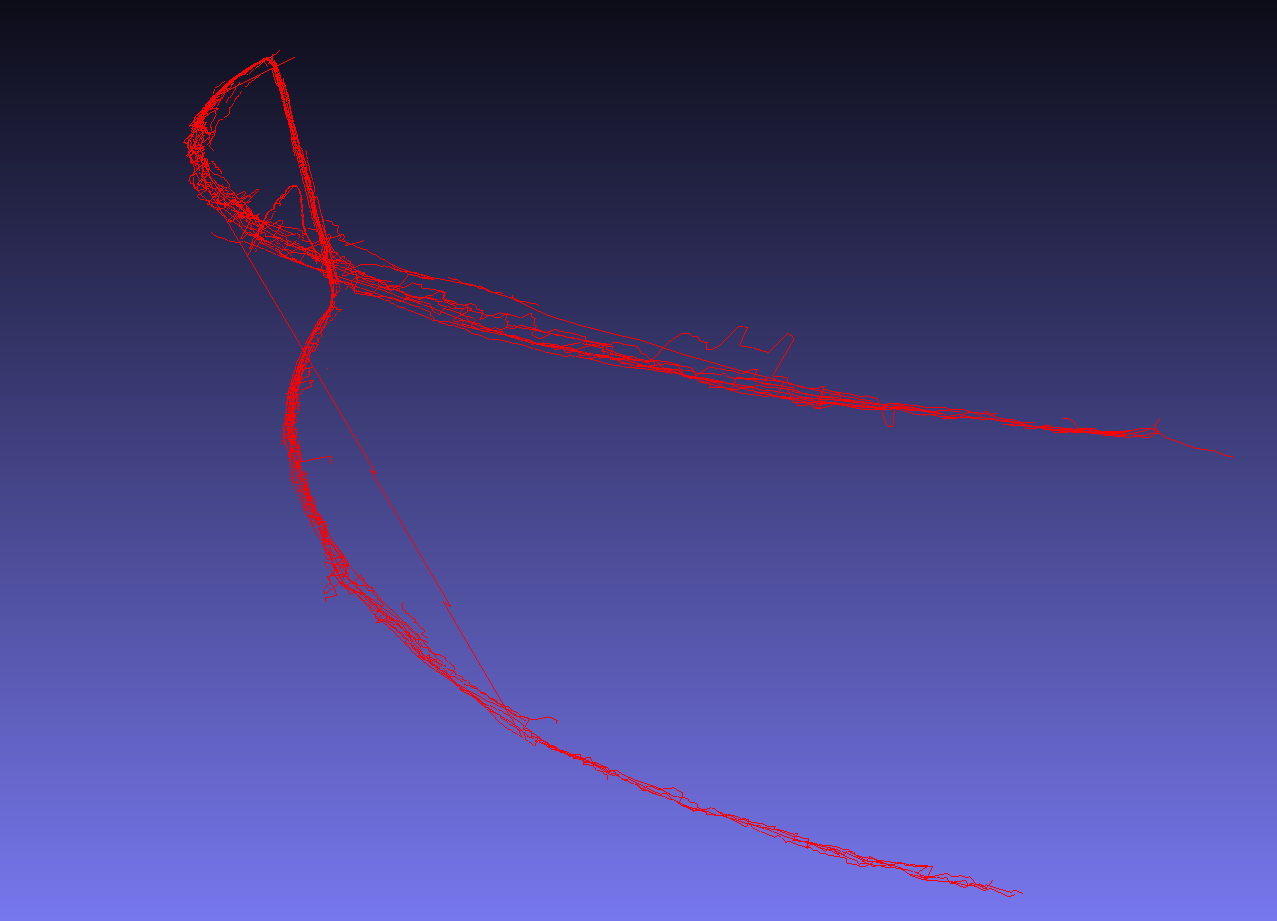
\includegraphics[width=0.2\linewidth]{figs/cluster32-2.png}\\
%%%%%     		&
%%%%%     		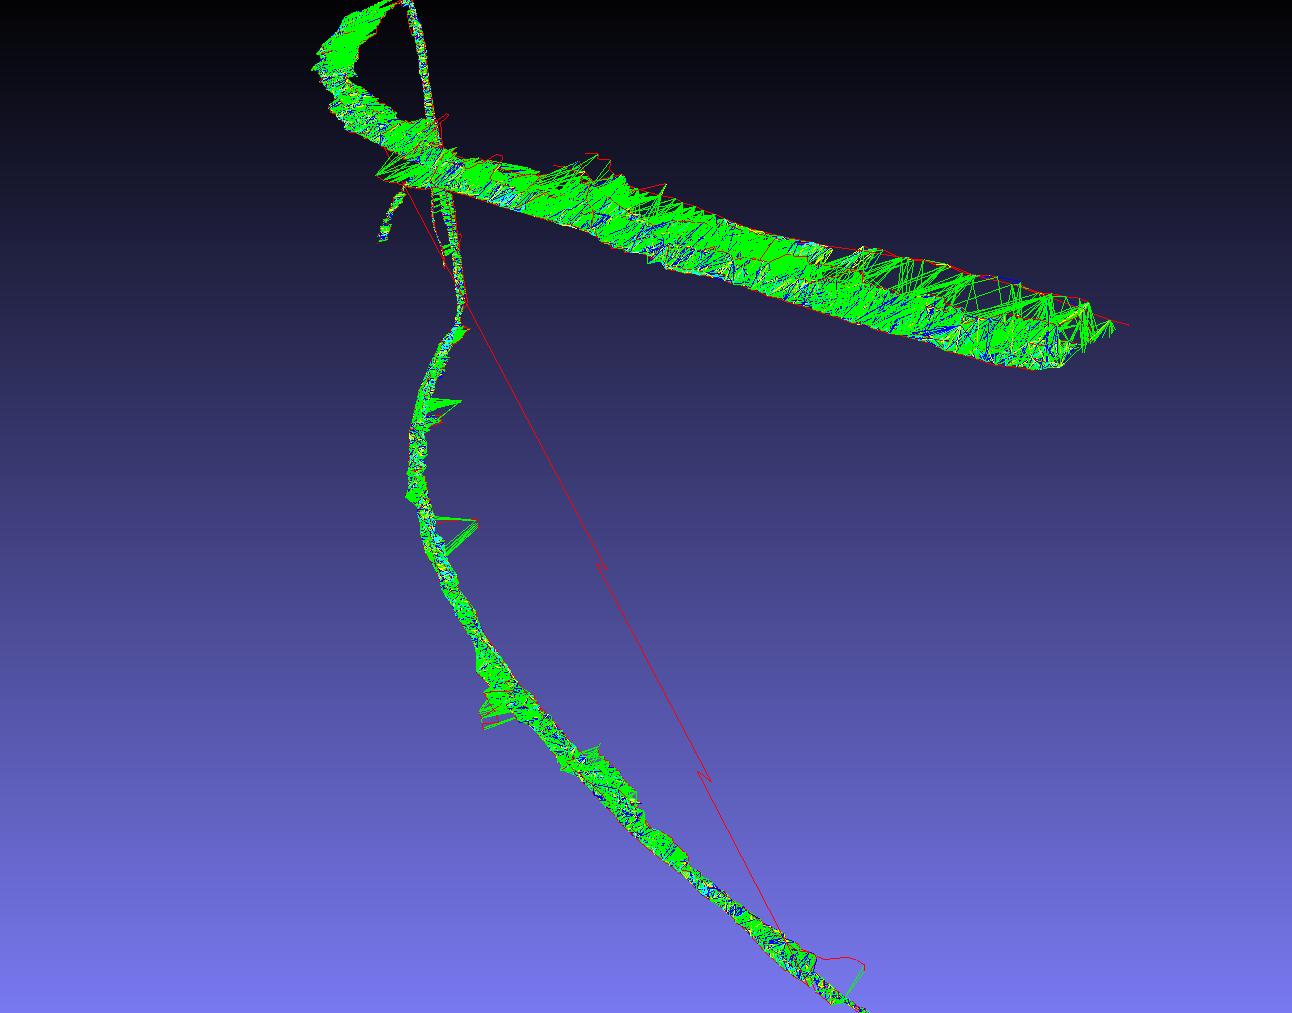
\includegraphics[width=0.2\linewidth]{figs/cluster32-corr2.png}
%%%%%     	\end{tabular}
%%%%%       \vspace{2em}
%%%%%     	\caption{The four bottlenecks of
%%%%%     		Fig.~\ref{fig:issues:remaining} are resolved by integration of
%%%%%     		information/cues from all views. (a) The shared supporting edges, which are marked with circles, create the purple links between the corresponding samples of the 3D curves. These purple bonds will then be used to pull the redundant segments together and reorganize the 3D model into a clean 3D graph. Observe how the determination of common	image support can identify portions of the green and blue curves as identical	while differentiating the red one as distinct. A real example for a bundle of related curves is shown in (b) and the links among their edges in (c).
%%%%%     	}
%%%%%     	%   based on which 3D information with a
%%%%%     	%   common cause can be integrated, leading to a four-stage process of $(i)$
%%%%%     	%   establishing the links as pictured above, $(ii)$ identifying portions of 3D
%%%%%     	%   curves which arise from the same source, Fig~\ref{fig:overlap:masks}, $(iii)$
%%%%%     	%   precise localization for 3D curves with a common cause,
%%%%%     	%   Fig~\ref{fig:graph:organization}a, (iv) Topological merging of these
%%%%%     	%   segments, leading to a topological graph of 3D curve segments,
%%%%%     	%   Fig~\ref{fig:graph:organization}e.}\label{fig:master:figure}
%%%%%     \end{figure}
%%%%%     
%%%%%     %\vspace{-0.3cm}
%%%%%     
%%%%%     \textbf{Multiview Curve-level Consistency Network:}
%%%%%     The identification of 3D edges sharing 2D edges leads to
%%%%%     high recall operating point with many false links due to accidental alignment of
%%%%%     edge support. False positives can be reduced without affecting high
%%%%%     recall by employing a notion of curve context for each 3D edgel: a link
%%%%%     between two 3D edgels based on a supporting 2D edgel is more effective if
%%%%%     the respective neighbors of the underlying 3D edge on the underlying 3D curve
%%%%%     are also linked. 
%%%%%     
%%%%%     The curve context idea requires establishing new pairwise links between 3D
%%%%%     curves using MLN, when there are a sufficient number of links with
%%%%%     $\phi_{ij}>\tau_{\epsilon}$ between their constituent 3D edges (in our
%%%%%     implementation, $\tau_{\epsilon}=3$ and we require 5 such edges or more). The
%%%%%     linking of 3D curves is represented by the Multiview Curve-level Consistency
%%%%%     network (MCCN), a graph whose nodes are the 3D curves $\Gama_j$ and the edges
%%%%%     represent the presence of high-weight 3D edge links between these 3D curves. The
%%%%%     \mccn graph allows for a clustering of 3D curves by finding connected
%%%%%     components; and once a link is established between two curves, there is a high
%%%%%     likelihood of their edges corresponding in a regularized fashion, thus
%%%%%     fewer common supporting 2D edges are required to establish a link between all
%%%%%     their constituent 3D edges. This fact is used to perform gap filling, since even
%%%%%     no edge support is acceptable to fill in small gaps and create a continuous and
%%%%%     regularized correspondence if both neighbors of the gap are connected (see
%%%%%     pseudocode in Supplementary Materials for details). The two stages in
%%%%%     tandem, \ie, high recall linking of 3D edges and use of curve context to reduce
%%%%%     false positives leads to high recall and high precision, \textit{i.e.}, all the
%%%%%     3D edges which need to be related are related and very few outlier connections
%%%%%     remain.
%%%%%     
%%%%%     \begin{figure}
%%%%%     	\captionsetup[subfigure]{labelformat=empty}
%%%%%     	\centering
%%%%%     	\begin{tabular}{cc}
%%%%%     		\multirow{2}[2]{*}[13mm]{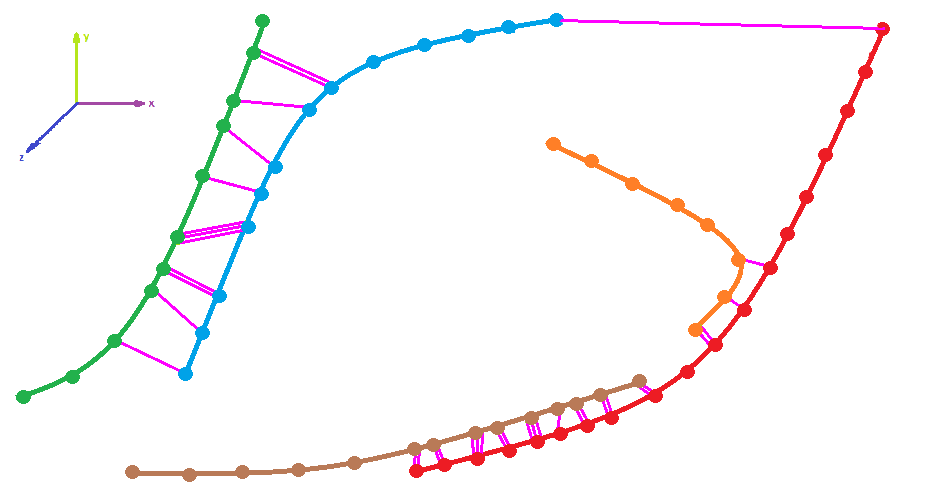
\includegraphics[width=0.55\linewidth]{figs/need-for-clusters.png}} &
%%%%%     		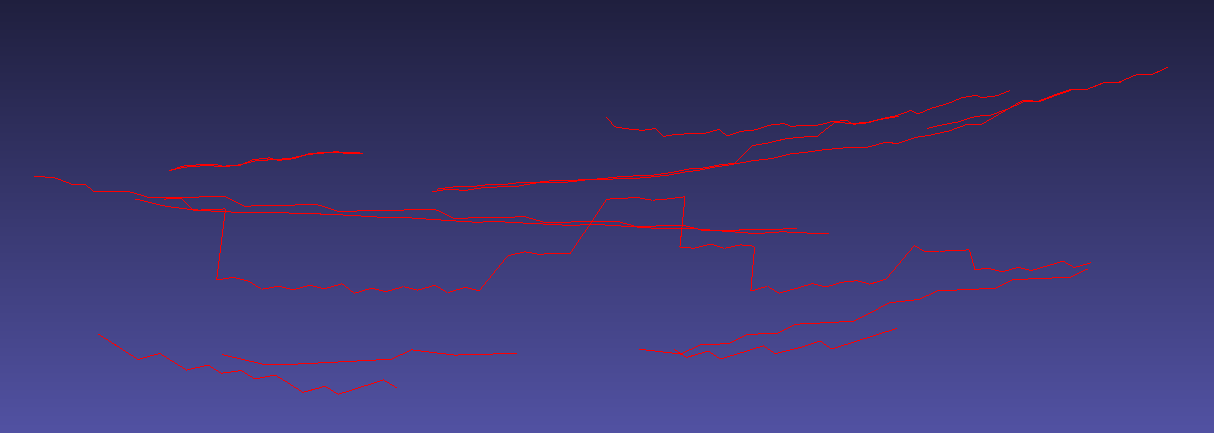
\includegraphics[width=0.45\linewidth]{figs/cluster7.png}\\
%%%%%     		&
%%%%%     		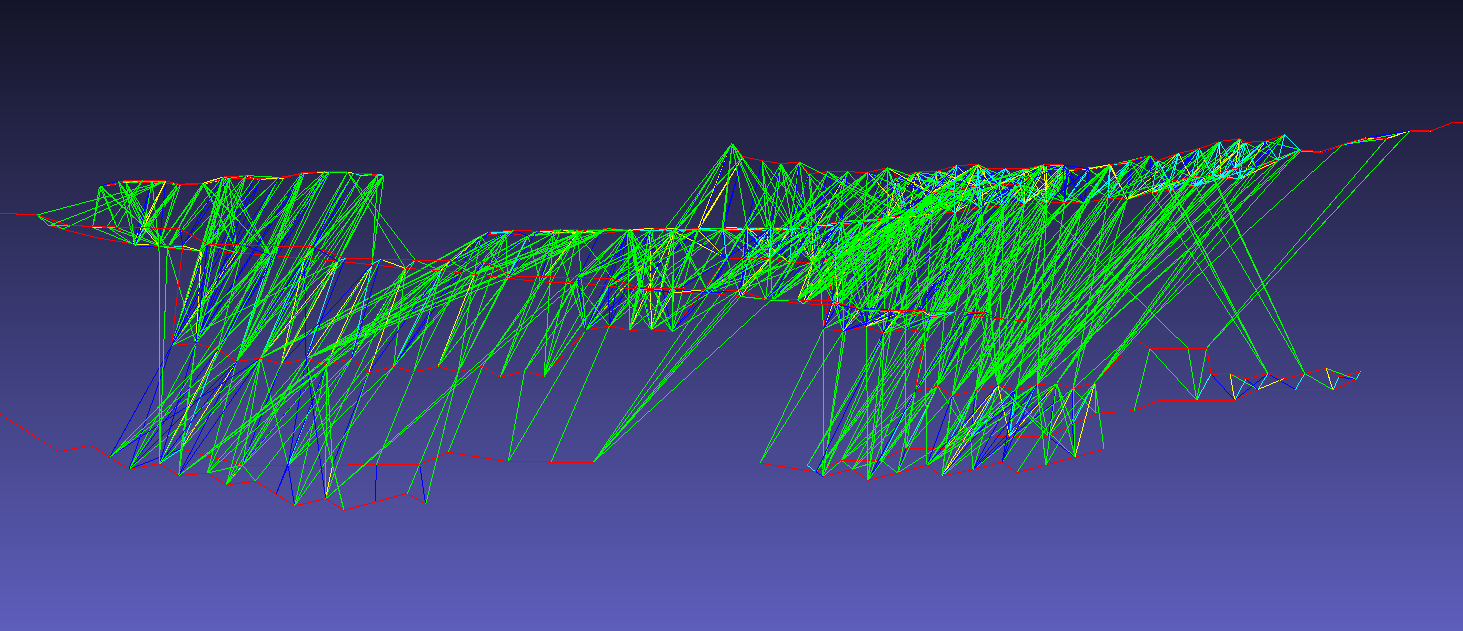
\includegraphics[width=0.45\linewidth]{figs/cluster7-corr.png}
%%%%%     		\\
%%%%%     	\end{tabular}
%%%%%     	%\ReduceBeforeCaptionfigspace
%%%%%     	\caption{\small 
%%%%%     		The correspondence between 3D edge samples is skewed along a curve, a direct indication that these links cannot be used as-is when averaging and fusing redundant curve reconstructions. Instead, each point is assumed to be in correspondence with the point closest to it on another overlapping curve, during the iterative averaging step. Observe that corrections can be partial along related
%%%%%     		curves.
%%%%%     	}
%%%%%     	\label{fig:overlap:masks}
%%%%%     \end{figure}

%\vspace{-0.3cm}

%The links between two 3D curves that are consistently overlapping according to
%evidence from multiple views form the so-called Multiview Curve-level
%Consistency Network, a graph defined as follows.
%\begin{definition}
%The Multiview Curve-level Consistency Network (MCCN) is a graph 
%\begin{equation}
%\text{\textit{MCCN}} = (S, L),
%\end{equation}
%where the vertices $S = \{1,\dots,K\}$ encode the set of 3D curves
%$\{\Gama_1,\dots,\Gama_K\}$ and $L$ is the link set defined below.
%\end{definition}
%\begin{definition}
%Let the set of so-called strong local links between curves $\Gama_i$ and
%$\Gama_j$ be defined as
%\begin{equation}
%S_{ij} \doteq \{(s,t) : \phi_{ij}(s,t) \geq \tau_{s}, \phi_{ij} \in
%\text{MLN}(\Gama_1,\dots,\Gama_K) \}.
%\end{equation}
%Then the set $L$ of the MCCN is defined as
%\begin{equation}
%L = \{(i,j) : |S_{ij}| \geq \tau_{sl}\}.
%\end{equation}
%\end{definition}
%\indraftnote{We can formulate L as an integral over alignment parameter, see
%rics notes}

%We cluster the 3D curves by computing the connected components of their MCCN.
%We then go back to local correspondences by filling-in short correspondence gaps
%of the MLN induced by the confidence gained by the curve-level consistency link.
%Further details are available in the form of a pseudocode in supplementary material.


%in this way, the set of these primitives is not an
%arbitrary heuristic but rather is a complete set of basic operations capable of
%breaking any merging problem into smaller chunks.

%\vspace{-0.8cm}

%\subsection{Other objectives}
%\begin{itemize}
%\item Help with the book to be published
%\item Take part in helping teach a graduate-level course.
%\end{itemize}

%\paragraph{Impact}

\section{Justificativa: as vantagens das curvas}
Além de possibilitarem as inúmeras aplicações do sistema proposto citadas no início da
Introdução, as curvas como \emph{features} básicas para reconstrução 3D e
calibração têm as seguintes vantagens.  As curvas provenientes de
descontinuidade de bordas nas imagens são mais densas e mais bem-estruturadas do
que pontos isolados, e representam eficientemente a imagem ou cena 3D
subjacente. Elas fornecem um bom compromisso entre uma representação altamente
redundante na forma de arrays de píxels, e uma representação altamente esparsa
das nuvens de pontos de interesse. Isso permite o cálculo rápido de
reconstruções 3D (os \emph{3D curve sketch}), que, apesar de não possuirem
superfícies explícitas, são ainda reconhecíveis, estruturadas, e de eficiente
manipulação e armazenagem. Essa eficiência representacional é evidenciada em
uma tendência recente em computação gráfica de usar renderizações baseadas em
curvas (\emph{line-based} rendering) para aplicações de internet que exigem
eficiência, e também por razões estéticas. A riqueza estrutural de curvas é
illustrada pelo fato de ser impossível registrar uma nova imagem não-calibrada
com relação a uma nuvem de pontos 3D por si só, ao passo que essa tarefa se
torna possível com curvas 3D dada a maior estruturação geométrica (\eg,
reprojetando-se as curvas 3D na nova imagem e alinhando-as às curvas detectadas
na imagem). Ademais, é bem sabido que representações baseadas em bordas
representam eficiente o conteúdo de uma imagem, o que motiva uma reconstrução de
curvas 3D eficiente para armazenar a informação geométrica mais relevante de uma
cena 3D. Curvas também têm maior invariância do que pontos de interesse a
mudanças de iluminação, são mais estáveis sob uma maior separação entre as
imagens, e são mais precisamente localizadas na direção normal. Ademais,
estrutura de curvas de bordas em uma imagem é correlacionada com propriedades
das superfícies subjacentes: curvas estacionárias (como as de reflectância) são
condições de contorno para reconstrução de superfícies, e a variação de
contornos de oclusão sob diferentes pontos de vista indica a curvatura da
superfície

\paragraph{Impacto tecnológico.} 
As reconstruções 3D propostas, que vão além de núvem de pontos, têm impactos em
aplicações que trabalho com cenas e objetos com baixa textura, como nos casos de
objetos feitos pelo homem: cenas urbanas, cenas \emph{indoors}, carros, peças
mecânicas, etc. Um exemplo são projetos provenientes do pioneiro Hololens da
Microsoft~\cite{nurutdinova2015towards}, bem como o sistema de visão 3D de robôs 
e carros autônomos.


\section{Metas}
\paragraph{Elaboração de Publicações}
Como metas específica deste projeto, tem-se a elaboração de
publicações (idealmente 1 ou mais por ano) nas principais revistas e conferências da área. Dentre as
revistas visadas, temos: International
Journal of Computer Vision, IEEE Pattern Analysis and Machine Intelligence, IEEE
Transactions in Image Processing, Pattern Recognition, ACM Computing Surveys, e
Journal of Mathematical Imaging and Vision. Também pretende-se enviar trabalhos
completos (arigos) às mais importantes conferências na área, a saber: IEEE CVPR
(Computer Vision and Pattern Recognition), IEEE ECCV (European Conference in
Computer Vision), IEEE ICCV (International Conference in Computer Vision),  ACM
SIGGRAPH, e o IEEE SIBIGRAPI. Por se tratar de uma pesquisa interdisciplinar,
também pretende-se publicar em periódicos em matemática pura, matemática aplicada
e análise numérica.


\section{Metodologia}
A execução do projeto será dividida nas seguintes frentes, visando atingir as
metas descritas na seção anterior, na ordem descrita na próxima seção:
\begin{itemize}
\item \textbf{Estudo de reconstrução 3D usando geometria diferencial e equações
  diferenciais} 
  Será estudado o trabalho do prof.\ Fabbri~\cite{fabbri2016multiview},
  bem com o trabalho do prof.\ Olver~\cite{Kogan:Olver:LobachevskiiJMA2015},
  procurando unir a generalidade à profundidade de resultados de cada técnica.
  Ao mesmo tempo, a teoria necessária para a compreensão de ambos os artigos
  será estudada.
\item \textbf{Estudo e co-autoria dos preprints de Peter Olver.} 
  Serão estudados e, possivelmente, co-autorados, dois preprints (não publicados), enviados por Peter Olver ao
  prof.\ Fabbri~\cite{Olver:Outline:Preprint:2020,Olver:Reprojn:Preprint:2020}. Ambos lidam com a reconstrução 3D das superfícies de objetos
  como um problema de reconstrução de sinais a partir de assinaturas ligadas a
  a invariantes. Nesse sentido, também será aprofundada Geometria Riemanniana,
  equações diferenciais e grupos de Lie.
\item \textbf{Estudo de Mapas de Difusão e Teoria de Padrões.} 
  Para se atingir uma solução global e para que se possa modelar certos
  parâmetros aprendendo-se de exemplos (dados), o aluno irá estudar o livro de
  Moura Neto e Fabbri sendo escrito sobre Mapas de Difusão e modelagem
  computacional.
\item \textbf{Validação e Experimentos de Larga escala.} Pretende-se realizar
experimentos na reconstrução em larga escala de objetos industriais 
partir de milhares de fotografias ou quadros de vídeo. A validação será
realizada através de comparaçao com objetos conhecidos \emph{a priori}
e impressos em impressoras 3D. 
\item \textbf{Desenvolvimento de Software livre para Visão Computacional.}
Pretende-se continuar o desenvolvimento de software livre, como uma
forma de contribuir para a sociedade, angariar colaborações,
garantir um controle de qualidade, e disseminar a pesquisa. 
\item \textbf{Elaboração de Publicações como descrito nas metas.}
\end{itemize}


%\begin{center}
%\begin{tabular} {||r|c|c|c|c||}
%\hline
%\textbf{Stages (trimesters)} & 1 & 2 & 3 & 4 \\
%\hline
%Reproduce 3D Curve Sketch System& X &  & & \\
%\hline
%Reproduce 3D Curve Drawing System& X & X & & \\
%\hline
%Reproduce 3D Lofting System &   & X &  & \\
%\hline
%Build graphs for surface merging& X & X & X & \\
%\hline
%Large scale expermients&   &   & & X\\
%\hline
%Write Software & X & X & X & X\\
%\hline
%Publish Open Source Software &  &  & X & X \\
%\hline
%Publications &  & X & X& X\\
%\hline
%\end{tabular}
%\end{center}

\section{Cronograma das Atividades}
A tabela abaixo mostra o cronograma para as principais frentes de atuação descritas na
seção anterior. Para a execução deste projeto, o período foi dividido em etapas aproximadamente
anuais.
\begin{center}
\begin{tabular} {||r|c|c|c|c||}
\hline
\textbf{Etapas anuais do doutorado} & 2 & 3 & 4 \\
\hline
Estudo comparativo de~\cite{Fabbri:Kimia:IJCV2016} (prof. Fabbri)
e~\cite{Kogan:Olver:LobachevskiiJMA2015} & X &    & \\
\hline
Estudo e co-autoria dos preprints de Peter Olver~\cite{Olver:Reprojn:Preprint:2020,Olver:Outline:Preprint:2020} & X &    & \\
\hline
Estudo de Mapas de Difusão e Teoria de Padrões &  X & X &  \\
\hline
Experimentos de Larga Escala &     & X & X\\
\hline
Escrita de Software Livre &   X & X & X\\
\hline
Elaboração de Publicações &   X & X & X\\
\hline
\end{tabular}
\end{center}

\section{Conclusão}
Este projeto propõe o avanço do 
paradigma baseado em curvas e superfícies para reconstrução 3D e calibração de
câmeras, complementando as técnicas atuais baseadas em pontos, as quais estão
sendo usadas em larga escala. A tecnologia proposta extenderá a capacidade das
técnicas atuais, permitindo o processamento de uma maior variedade de objetos de
interesse industrial, ao mesmo tempo impondo menos restrições na aquisição. 
A pesquisa também irá alavancar a colaboração internacional com o matemático
Peter Olver, que também pesquisa visão computacional.


%\nocite{Fabbri:2002}
\addcontentsline{toc}{section}{Refer\^{e}ncias}
\bibliographystyle{ieeetr}
%\bibliography{personal,strings,shading,multiview,motion,Kimia,catagorization,edge-linking,deformable,medical,graphics,active-contours,texture,imaging,tracking,shape-papers,bib-header,video,math-books,math,psych-books,metric,edge,leymarie_pami_scaffold,vision-books,vision,nn-search,multidimscaling,psychophysics,indexing,segmentation,image-databases,shape-matching,neuro,skeleton,skeleton2D,aspect-graphs,recognition,surface-networks,ridge,proceedings,perceptual-grouping,continuation,graph-matching-2,cooper}
\bibliography{bib/fabbri-multiview,bib/fabbri-olver.bib,bib/kimia-multiview,bib/fabbri-machine-learning,bib/fabbri-vision,bib/fabbri-math-books,bib/fabbri-vision-books,bib/fabbri-video,bib/fabbri-recognition,bib/fabbri-indexing,bib/fabbri-proceedings,multiview,rf-multiview,Pajdla,ref}
%
% Assinaturas:
%\newpage
%\ \\\vspace{7cm}
%\center $\overline{\ \ \ Ricardo\ Fabbri\ \ \ }$
%\ \\\vspace{4cm}
%\center $\overline{\ \ \ Luciano\ da\ Fontoura\ Costa\ \ \ }$
  \includegraphics[width=0.5\linewidth]{figs/assinatura-cleuber.png}\\
  
\includegraphics[width=0.2\linewidth]{figs/signature-extensive.png}\\[-4em]
  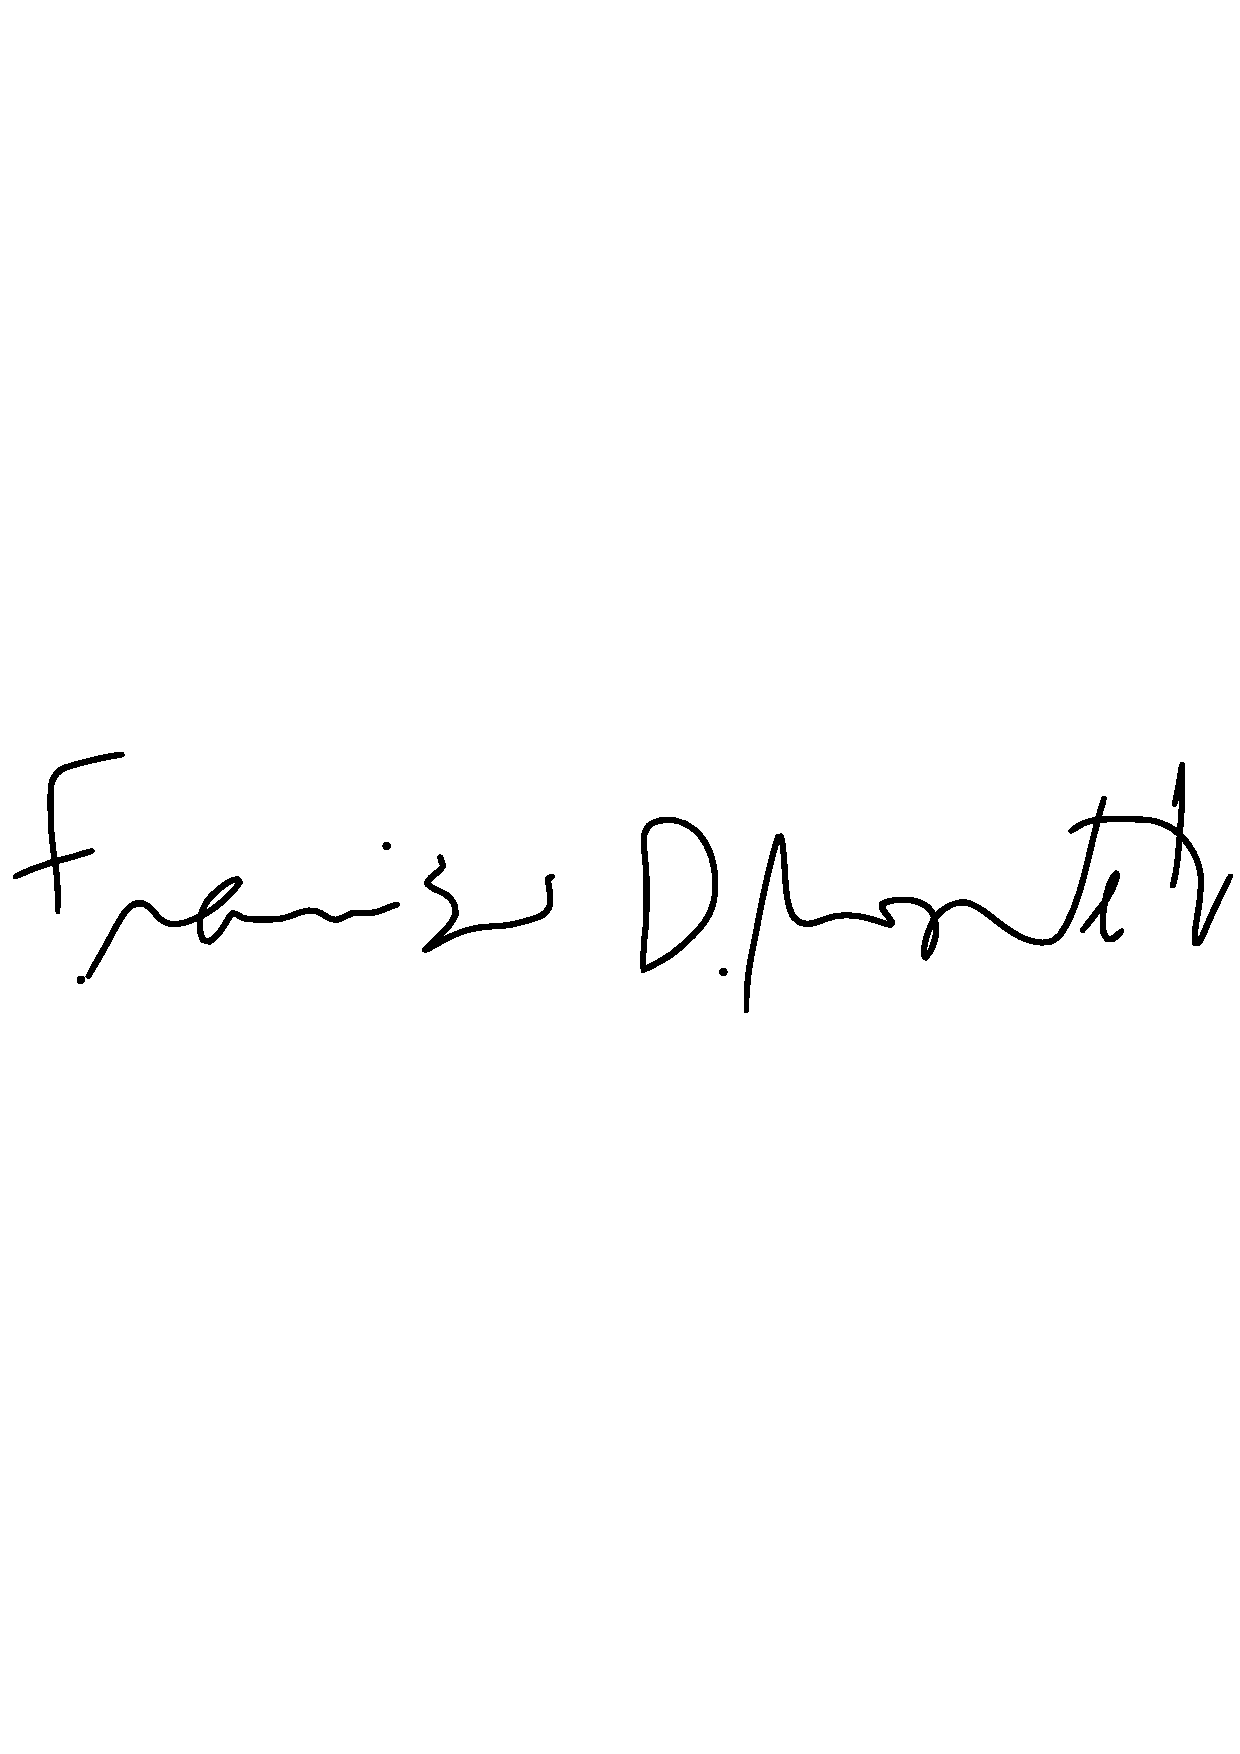
\includegraphics[width=0.2\linewidth]{figs/assinatura-francisco-moura-neto.pdf}
\end{document}
